
\chapter{Resultados Experimentais }
\label{cap:resultados}

\section{Resultados}





Seguindo requisitos de negócio da Intercement, uma primeira
bateria de testes foi feita pensando em como seria a realidade de um sistema de
predição usado em produção na fábrica. Dessa maneira, usamos os índices RC3 e
RC7 para modelar predições para o índice RC28. Como explicado na introdução, o
índice de resistência RCX é medido X dias após o lote de cimento é produzido. Ou
seja, é desejável se ter uma estimativa de um índice que demora semanas para
poder ser medido como o RC28. \\


Os testes foram realizados com modelos sequenciais e não sequenciais. Para ambos
as classes de modelos os dados foram transformados para possuirem variância
unitária e média 0. Os índices RC3 e RC7 foram usados como entrada e o índice
RC28 foi usado como saída. Os dados foram divididos em
\textit{treino}, \textit{teste} e \textit{validação}. Usamos os dados de treino
e teste para treinar os
modelos, e os de validação apenas para avaliar o seu erro. O
gráfico~\ref{fig:divrc28} mostra essa divisão. Lembramos que apenas os dados de
validação são inéditos para os modelos, com eles avaliamos a capacidade de
generalização dos modelos. 


\begin{figure}[H]
  \centering
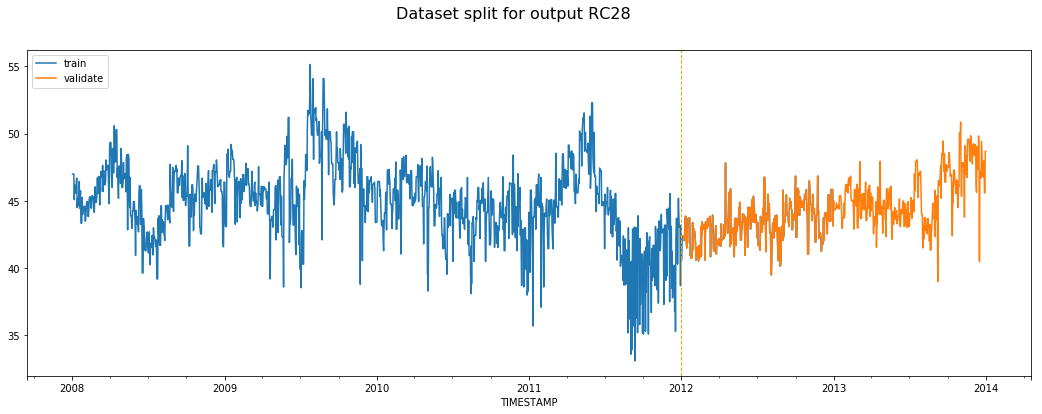
\includegraphics[width=0.9\columnwidth]{dataset_splitRC28.png}
\caption{Divisão do dataset para a saída RC28, os pontos azuis foram usados para
treino e os pontos laranjas usados para validação.}
  \label{fig:divrc28}
\end{figure}





Seguem então os resultados dos modelos não-sequenciais para esse experimento, os
erros indicados são calculados pela métrica R2: \\



\begin{figure}[H]
\centering
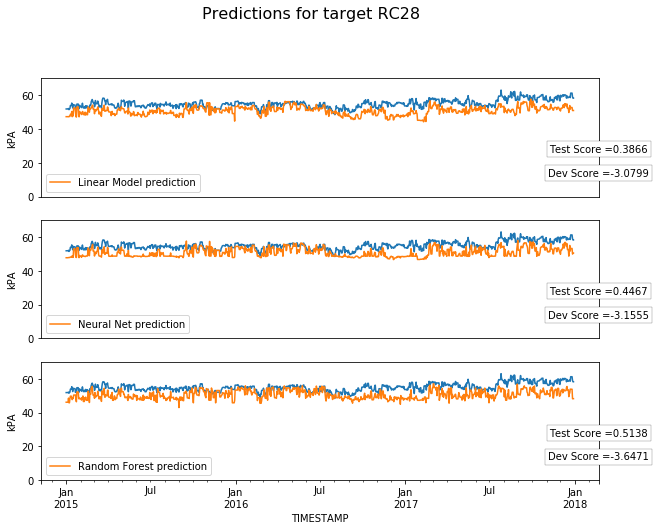
\includegraphics[width=0.9\columnwidth]{exped_saco_2008-2012-2014RC28.png}
\caption{Comparação dos 3 modelos não-sequenciais na tarefa de regressão do índice RC28}
\label{fig:3nseq}
\end{figure}



E os resultados para o modelo Encoder-Decoder-Forecaster: \\



%%% Local Variables:
%%% mode: latex
%%% TeX-master: "../quali"
%%% End:

